%%
%
% ARQUIVO: cap-01.tex
%
% VERSÃO: 1.0
% DATA: Maio de 2016
% AUTOR: Coordenação de Trabalhos Especiais SE/8
% 
%  Arquivo tex de exemplo de capítulo do documento de Projeto de Fim de Curso.
%
% ---
% DETALHES
%  a. todo capítulo deve começar com \chapter{•}
%  b. usar comando \noindent logo após \chapter{•}
%  c. citações para referências podem ser
%       i. \citet{•} para citações diretas (p. ex. 'Segundo Autor (2015)...'
%       ii. \citep{•} para citações indiretas (p. ex. '... (AUTOR, 2015)...'
%  d. notas de rodapé devem usar dois comandos
%       i. \footnotemark para indicar a marca da nota no texto
%       ii. \footnotetext{•}, na sequência, para indicar o texto da nota de rodapé
%  e. figuras devem seguir o exemplo
%       i. devem ficar no diretório /img e devem ser no formato EPS
%  f. tabelas devem seguir o exemplo
%  g. figuras e tabelas podem ser colocadas em orientação landscape
%       i. figuras: usar \begin{sidewaysfigure} ... \end{sidewaysfigure}
%                   em vez de \begin{figure} ... \end{figure}
%       ii. tabelas: usar \begin{sidewaystable} ... \end{sidewaystable}
%                    em vez de \begin{table} ... \end{table}
%  h. toda figura e tabela deve ser referenciada ao longo do texto com \ref{•}
% ---
%%

\chapter{Introdução}

\section{Motivação}
Cada vez mais as máquinas estão sendo utilizadas em atividades de nossa sociedade. Atuando na substituição de profissionais ou no auxílio dos mesmos, elas estão presentes e participando de nosso cotidiano ativamente. A implementação de sistemas de visão computacional tem se tornado, portanto, uma necessidade mais forte à medida que as aplicações que envolvem o tratamento de imagens se desenvolvem e buscam se aproximar da visão e da análise humana.
A segmentação é uma importante técnica utilizada nas atividades que envolvem o processamento digital de imagens. Diversas são as aplicações que fazem uso da identificação e análise de uma imagem, necessitando do estudo de regiões específicas das mesmas a fim de alcançar resultados e conclusões de forma eficiente.
Por se tratar de um problema sem solução universal e de vasta aplicação,  existem inúmeras possibilidades a serem exploradas e muito se tem estudado sobre essa área, com a evolução de novas técnicas e algoritmos que trazem uma nova abordagem ao problema.
%Esse projeto trará, portanto, um conhecimento mais profundo nesse importante domínio da Visão Computacional com a concepção de um produto que servirá tanto como base para estudo quanto uma base para futuros projetos mais avançados.
Esse projeto visa estudar e implementar técnicas de segmentação de imagens no ambiente Android, possibilitando o aprendizado de diferentes métodos da área de processamento de imagens, incluindo a área de visão computacional, bem como de desenvolvimento de aplicativos na plataforma Android. A Figura \ref{fig:tela_android} exibe o resultado do aplicativo que este projeto de final de curso está desenvolvendo.


% Figura -----------------------------------------------------------------------------------------------------------------------------
  \begin{figure}[!htb]
       \begin{center}  
          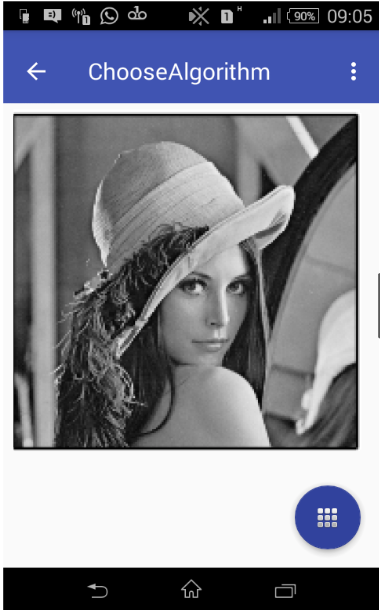
\includegraphics[width=0.2\columnwidth]{img/tela_android-original.png} \quad
          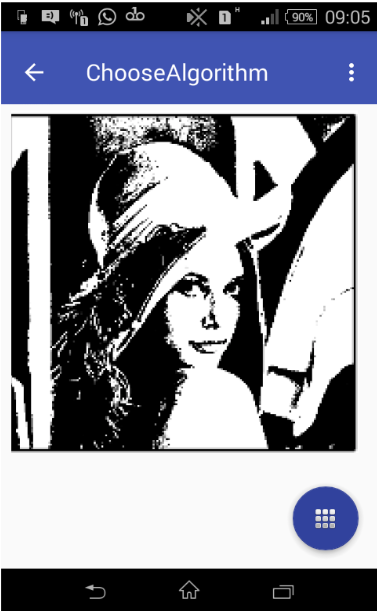
\includegraphics[width=0.2\columnwidth]{img/tela_android.png}
           \caption{\label{fig:tela_android}Tela do Aplicativo Android (imagem original e imagem segmentada).}
           % \vspace{2.0em}
       \end{center}
   \end{figure}
 % Figura -----------------------------------------------------------------------------------------------------------------------------

% um conhecimento mais profundo nesse importante domínio da Visão Computacional com a concepção de um produto que servirá tanto como base para estudo quanto uma base para futuros projetos mais avançados.


\section{Objetivos}
O objetivo dessa pesquisa é o desenvolvimento de uma aplicação móvel, em plataforma Android, capaz de segmentar imagens por meio de diferentes algoritmos e técnicas de pré-processamento na área de Visão Computacional. A realização de todas as etapas de desenvolvimento até a concepção do produto final, que será disponibilizado para livre utilização, permitirá aos alunos maior conhecimento nesse assunto que é um dos domínios mais promissores da tecnologia e complementará a sua formação como engenheiros de Computação. A Figura \ref{fig:diag_blocos} ilustra os passos do projeto, onde o aplicativo poderá adquirir imagens diretamente da câmera do dispositivo ou da galeria de imagens do dispositivo. O bloco denominado Pré-Processamento ilustra uma possível etapa de pré-processamento das imagens oriundas da câmera ou do banco de imagens, com a finalidade de tratar as imagens para os algoritmos de segmentação. O bloco seguinte, Técnicas de Segmentação implementa um ou mais métodos de segmentação, descritos no capítulo \ref{cap:segmentacao}. Finalmente, o bloco Exibição vai exibir a imagem segmentada na tela do dispositivo. 

% Figura -----------------------------------------------------------------------------------------------------------------------------
  \begin{figure}[!htb]
       \begin{center}  
          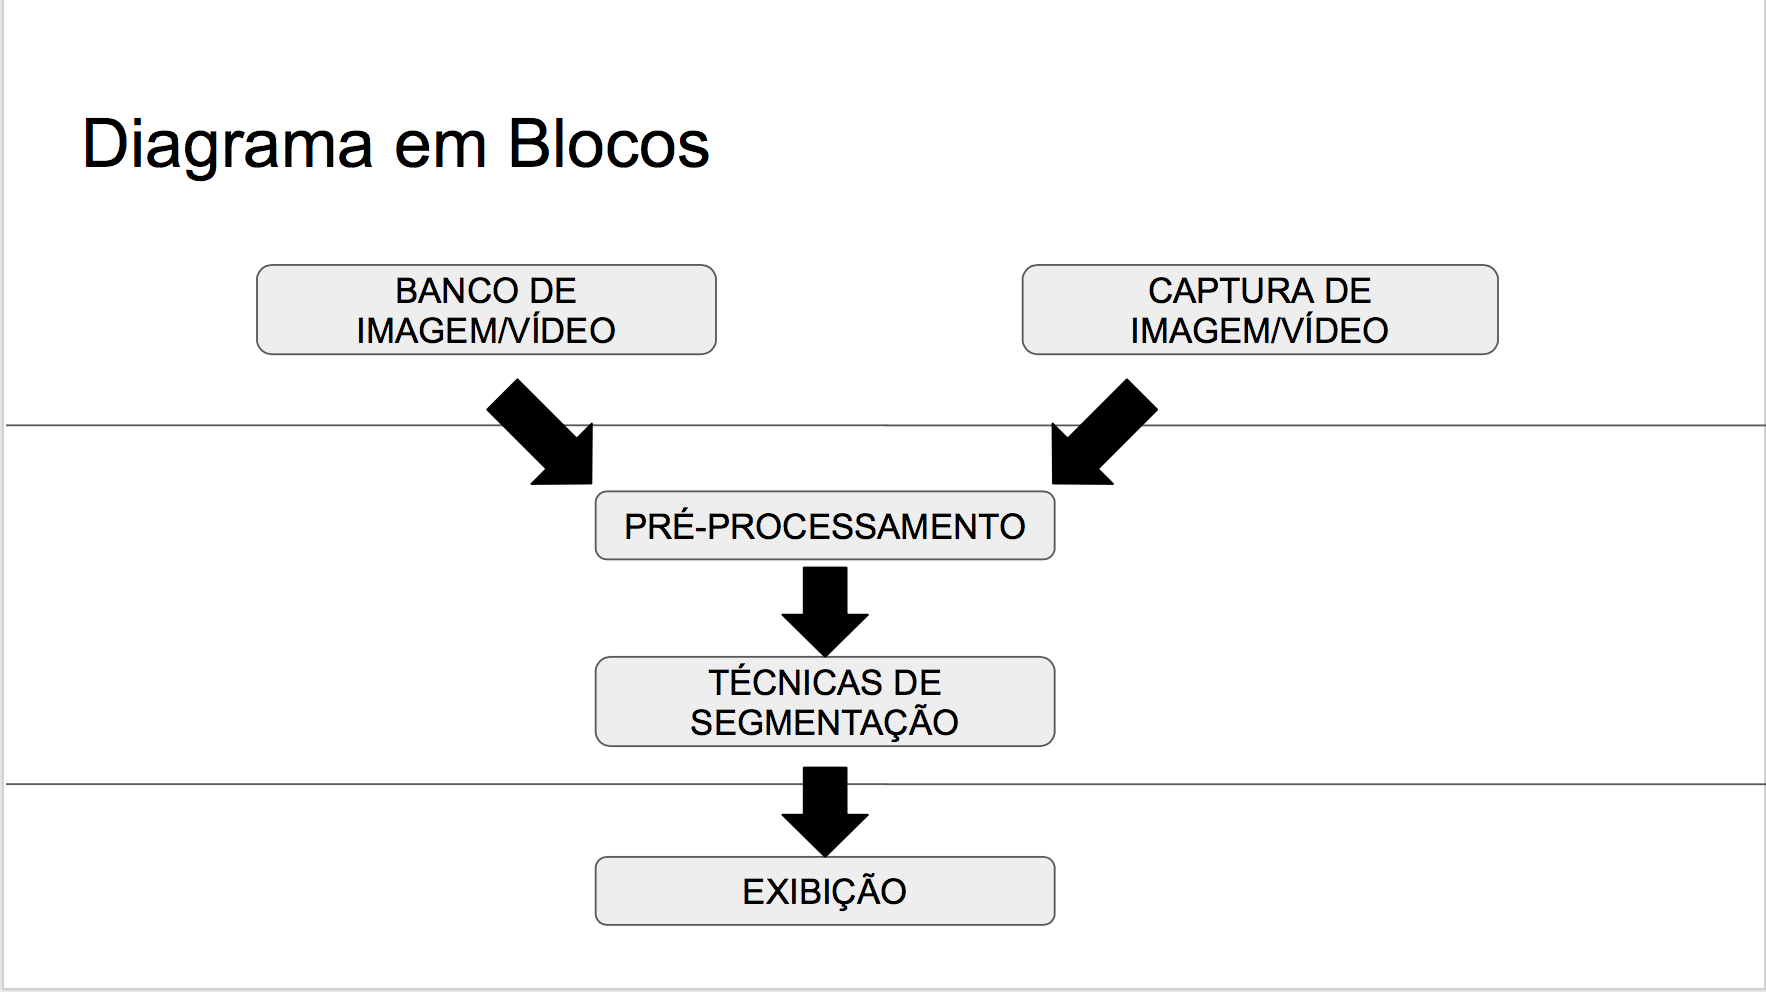
\includegraphics[width=0.7\columnwidth]{img/diag_blocos.png}
           \caption{\label{fig:diag_blocos}Diagrama em Blocos do Projeto.}
           % \vspace{2.0em}
       \end{center}
   \end{figure}
 % Figura -----------------------------------------------------------------------------------------------------------------------------


\section{Justificativa}
Este trabalho pode ser justificado com base nos seguintes pontos:
\begin{itemize}
\item Inexistência de uma solução única para o problema em questão. Trata-se de um problema ainda em aberto com muitas oportunidades a serem exploradas;
\item Diversas aplicações necessitam da segmentação de imagens como parte importante das suas atividades, além de outras que podem ser aprimoradas e desenvolvidas por meio de sua utilização;
\item Visão computacional como domínio promissor da tecnologia, com uma atuação cada vez maior no mercado e interação com outros domínios como robótica e inteligência artificial.
\end{itemize}


%\chapter{REFRÊNCIAS BIBLIOGRÁFICAS}
%\begin{itemize}
%    \item GLOCKSTEIN, Bob. Quadtrees and Octrees. Disponível em: <http://euklid.mi.uni-koeln.de/c/mirror/www.cs.curtin.edu.au/units/cg351-551/notes/lect51.html>. Acesso em: 10 mai. 2017
%    \item Chris. Segmentation. Disponível em: <http://www.bioss.ac.uk/people/chris/ch4.pdf>. Acesso em: 10 mai. 2017
%    \item STRAND, Robin. Segmentation. Disponível em: <http://www.it.uu.se/edu/course/homepage/\\bild1/ht14/L6\_segmentation.pdf>. Acesso em: 10 mai. 2017
%\end{itemize}





